% Koko
\documentclass[ichigo,normal,cn]{elegantnote}
\usepackage{tikz}
\definecolor{light-gray}{gray}{0.95}
\newcommand{\code}[1]{\colorbox{light-gray}{\texttt{#1}}}
\newfontfamily\courier{Courier New}
\lstset{linewidth=1.1\textwidth,
	numbers=left,
	basicstyle=\small\courier,
	numberstyle=\tiny\courier,
	keywordstyle=\color{blue}\courier,
	commentstyle=\it\color[cmyk]{1,0,1,0}\courier, 
	stringstyle=\it\color[RGB]{128,0,0}\courier,
	frame=single,
	backgroundcolor=\color[RGB]{245,245,244},
	breaklines,
	extendedchars=false, 
	xleftmargin=2em,xrightmargin=2em, aboveskip=1em,
	tabsize=4, 
	showspaces=false
	basicstyle=\small\courier
}
\title{程序设计实践课程作业 \\ 
Pastebin.rs 设计文档}
\author{2017211305 班 \\ 2017211240 于海鑫}

\begin{document}
\maketitle

\code{pastebin},又被称为\emph{文本存储网站},是一种存储纯文本的线上网站。通常用于存储代码片段或者日志等文本信息以供分享。最早的 \code{pastebin} 网站是 \code{pastebin.com} 大约在上世纪末出现,现在仍活跃在互联网中。国人最常用的 \code{pastebin} 网站应该是 \textbf{Ubuntu Pastebin},其界面比较简陋,且无法很好的支持手机端的访问。

在程序设计实践这门课的课程作业中,我们使用 \textbf{Rust} 作为编程语言,实现了一款类似 \textbf{Ubuntu Patebin} 的文本存储网站。同时添加了账户以及分享链接等功能,以方便用户的使用。我们的项目命名为 \textbf{Pastebin.rs},以 \texttt{GPLv3} 协议开源,托管在 \code{github.com} 上,链接为 \texttt{https://github.com/name1e5s/pastebin.rs}。

\section{概览}

\subsection{设计需求}
设计一个代码存储网站,可以支持用户创建新代码片段、查看他人创建的代码片段。

除此之外,改网站还应包含如下功能:
\begin{itemize}
    \item 提供基本的代码高亮功能,方便用户查看代码
    \item 允许用户匿名创建新片段,对于未登录用户来说只能创建匿名代码片段
    \item 提供 API 服务,方便第三方服务进行调用
\end{itemize}

\subsection{编程环境}

操作系统: KUbuntu 19.10

编程语言:Rust

开发环境:VS Code

\section{API 设计}

我们一共提供如下 7 个 API。

\begin{itemize}
    \item \code{POST(/api/register)}\ 注册新账户
    \item \code{POST(/api/login)}\ 登录
    \item \code{POST(/api/login)}\ 注销
    \item \code{POST(/api/new)}\ 新建 Paste
    \item \code{GET(/api/qr/:id)}\ 获取 Paste 的二维码
    \item \code{GET(/api/user/:username)}\ 获取某用户的全部 Paste
    \item \code{GET(/api/paste/:id)}\ 获取某 Paste 的全部信息
\end{itemize}

\section{数据库设计}

根据需求,我们发现我们需要设计一个用户表来保存用户相关的信息,一个代码片段表来保存用户提交的代码片段。除此之外,为了方便第三方 API 的接入,我们引入一个 \code{TOKEN} 表来保存 TOKEN 和用户之间的联系。

创建表的代码如下:

\begin{lstlisting}
-- users table
CREATE TABLE users (
    username TEXT PRIMARY KEY NOT NULL UNIQUE,
    password TEXT NOT NULL
);

CREATE TABLE api_tokens (
    token UUID PRIMARY KEY NOT NULL,
    user_name TEXT NOT NULL,

    FOREIGN KEY (user_name) REFERENCES users(username) ON DELETE CASCADE
);

CREATE TABLE pastes (
    id UUID PRIMARY KEY NOT NULL,
    title TEXT,
    lang TEXT NOT NULL,
    content TEXT NOT NULL,
    author_name TEXT NOT NULL,
    created_at TIMESTAMP NOT NULL,

    FOREIGN KEY (author_name) REFERENCES users(username) ON DELETE CASCADE
);

INSERT INTO users VALUES ('Anonymous', ' ');
INSERT INTO users VALUES ('test', 'password');
\end{lstlisting}

\section{模块划分}
我们的项目分为三层,从下到上分别为数据访问层,服务层以及界面层。上层可以调用下一层提供的 API,但下一层无法调用上一层的函数。

\subsection{数据访问层}
在这一层中,我们对数据库的表进行了抽象。提供了一些基础的增删查改操作的 API 以供上层调用。这一层主要包含如下几个结构:

\subsubsection{User}

定义如下:

\begin{lstlisting}
#[derive(Debug, Serialize, AsChangeset, Queryable)]
pub struct User {
    username: String,
    #[serde(skip_serializing)]
    password: String,
}
\end{lstlisting}

其是对数据库内的 \code{users} 表的进一步封装,用以表示在网站内注册的用户。除了基础的 \code{getter} 以及 \code{setter} 之外,\textbf{User} 类还提供了如下几个方法。

\paragraph{pub async fn get\_user(name: String, pool: \&ConnPool) -> Result<Self, Error>}
根据用户名查找用户。当用户存在时,返回 \code{Ok(Self)} 表示当前用户存在,并返回用户的具体信息;如果用户不存在,返回 \code{Err(Error)},表示用户不存在。当查找出错时也会返回 \code{Err(Error)} 但是返回的 \code{Error} 信息可能会不同。

\paragraph{pub async fn delete(self, pool: \&ConnPool) -> Result<usize, Error>}
从数据库中删除当前用户,如果删除成功,会返回一个 \code{Ok(usize)} 以表示删除成功,返回的数值为删除后表内的用户数。如果删除失败就返回 \code{Err(Error)}, 内部包含错误的详细信息。

\paragraph{pub async fn new\_token(self, pool: \&ConnPool) -> Result<APIToken, Error>}
创建一个与用户相关联的 \code{token} 并返回。

\paragraph{pub async fn insert(self, pool: \&ConnPool) -> Result<User, Error>}
这实际上是与之相关联的 \textbf{NewUser} 的方法,其作用是插入一个新的用户,如果成功插入,则返回插入的用户的信息。否则报错。

\subsubsection{APIToken}
表示与用户关联的 \code{Token} 信息。其定义如下:
\begin{lstlisting}
#[derive(Debug, Serialize, Identifiable, Queryable, Associations, Insertable)]
#[table_name = "api_tokens"]
#[primary_key(token)]
pub struct APIToken {
    token: APITokenID,
    user_name: String,
}
\end{lstlisting}
这一 \code{Token} 信息用于全部需要登陆的 API 中,以此可以校验用户的身份,因为其使用标准的 UUID 规范来生成,直接碰撞到 Token 的可能性几乎为 0。

除了基础的 \code{getter} 以及 \code{setter} 之外,\textbf{APIToken} 类还提供了如下几个方法。

\paragraph{pub async fn get\_token(id: APITokenID, pool: \&ConnPool) -> Result<Self, Error>}
根据  \code{Token} 的 UUID 获取  \code{Token} 的结构体。如果  \code{Token} 不存在会报错。

\paragraph{pub async fn check\_token(id: APITokenID, pool: \&ConnPool) -> bool}
判断 \code{Token} 是否存在。

\paragraph{pub async fn delete(self, pool: \&ConnPool) -> Result<usize, Error>}
删除 \code{Token},用以实现注销操作。

\paragraph{pub async fn insert(self, pool: \&ConnPool) -> Result<APIToken, Error>}
插入一个新的 \code{Token},用以实现登录操作,如果成功插入,则返回插入的用户的信息。否则报错。

\subsubsection{Paste}

\begin{lstlisting}
#[derive(Debug, Serialize, Deserialize, AsChangeset, Identifiable, Queryable, Insertable)]
#[table_name = "pastes"]
pub struct Paste {
    id: PasteID,
    title: Option<String>,
    lang: String,
    content: String,
    author_name: String,
    created_at: chrono::NaiveDateTime,
}
\end{lstlisting}

其是对数据库内的 \code{pastes} 表的进一步封装,用以表示在网站内注册的用户。除了基础的 \code{getter} 以及 \code{setter} 之外,\textbf{Paste} 类还提供了如下几个方法。

\paragraph{pub async fn get\_paste\_by\_id(paste\_id: PasteID, pool: \&ConnPool) -> Result<Self, Error>}
根据  \code{Paste} 的 UUID 获取  \code{Paste} 的结构体。如果  \code{Paste} 不存在会报错。

\paragraph{pub async fn get\_paste\_list\_by\_user\_name()}
根据用户名获取其名下的全部 \code{Paste}。如果用户不存在会报错。

\paragraph{pub async fn insert(self, pool: \&ConnPool) -> Result<Self, Error>}
插入一个新的 \code{Paste} 进入表内。

\subsection{服务层}

这一层是在下一层的基础上对业务逻辑进行了封装,同时这一层提供了 API 服务。
这一层内的函数的返回值相同,都是 \code{APIResponse},其定义如下:

\begin{lstlisting}
pub enum APIResponse<T, E> {
    Valid(T),
    Invalid(E),
}
\end{lstlisting}

当函数返回 \code{Valid(T)} 时,表示成功输出结果,返回真实数据,否则返回错误码以及可能的出错原因。

这一层可以分为如下几个模块。

\subsubsection{User}
这个模块内主要是对于用户相关的函数。仅有的两个函数如下:

\paragraph{pub async fn register(mut req: Request<ConnPool>) -> Result}
注册,根据请求的用户名字和密码建立新账户。

\paragraph{pub async fn login(mut req: Request<ConnPool>) -> Result}
登录,使用给定的账户名和密码登录账户,如果成功则返回一个 \code{Token} 以及用户名。

\paragraph{pub async fn logout(mut req: Request<ConnPool>) -> Result}
注销给定的 \code{Token},以此实现用户的登出操作。

\subsubsection{Paste}
这个模块内主要是代码片段相关的函数。

\paragraph{pub async fn get(req: Request<ConnPool>) -> Result}
根据 Paste 的 ID 获取 Paste 全文。

\paragraph{pub async fn list(req: Request<ConnPool>) -> Result}
获取某一用户的全部 Paste。

\paragraph{pub async fn new(mut req: Request<ConnPool>) -> Result}
新建一个 Paste。

\paragraph{pub async fn get\_qrcode(
    req: Request<ConnPool>,
)}
根据给定的 ID 返回访问该 ID 对应的页面的二维码文件。

\subsection{界面层}
这一层的主要作用是根据服务层提供的 API 配合网页模板完成网页生成的过程,函数如下。

\paragraph{pub async fn get(req: Request<ConnPool>) -> Response}
生成指定 ID 的 Paste 的网页。

\paragraph{pub async fn new(req: Request<ConnPool>) -> Response}
生成新建 Paste 的网页。

\paragraph{pub async fn list(req: Request<ConnPool>) -> Response}
生成用户下全部 Paste 的网页。

\section{实现}

我们使用 \code{Rust} 进行了整改服务器部分的实现。

\subsection{异步化}
我们使用了 Rust 官方开发的 \code{tide} 库作为我们核心库。\code{tide} 是对 \code{HTTP} 库的一个异步化的简单封装。作为官方实现的库,其对最近加入 Rust 的 \code{async/await} 语法有着很好的支持。得益于此,我们的程序在设计之初就考虑了如何异步化,最总达成了一个很好的\code{异步化}服务器。

\subsection{线程池}
Rust 的 \code{async} 函数最终的返回值是一个带有 \code{Future} Trait 的对象,为了让这个对象能够执行我们需要一个执行者来进行这一操作。我们最终使用 \code{async-std} 作为我们的执行者。

\code{async-std} 的底层实现其实是一个带有任务窃取的线程池搭配 \code{epoll} 操作实现的高效轮询,以此很好地实现了线程的复用以及任务的调度。

\subsection{连接池}
我们使用 \code{r2d2} 提供的通用连接池实现了一个支持泛型的连接池,该连接池可以方便地跨线程共享,还支持将查询操作异步化,大幅提升了服务器的效率。

\subsection{错误处理}
我们构造了统一的 \code{Error} 结构来处理我们的全部错误。

\section{运行效果}

我们将该程序部署到了我们的阿里云服务器上面,网址为 \code{http://name1e5s.fun:8888/},主界面效果如:

\begin{figure}[!htbp]
    \centering
    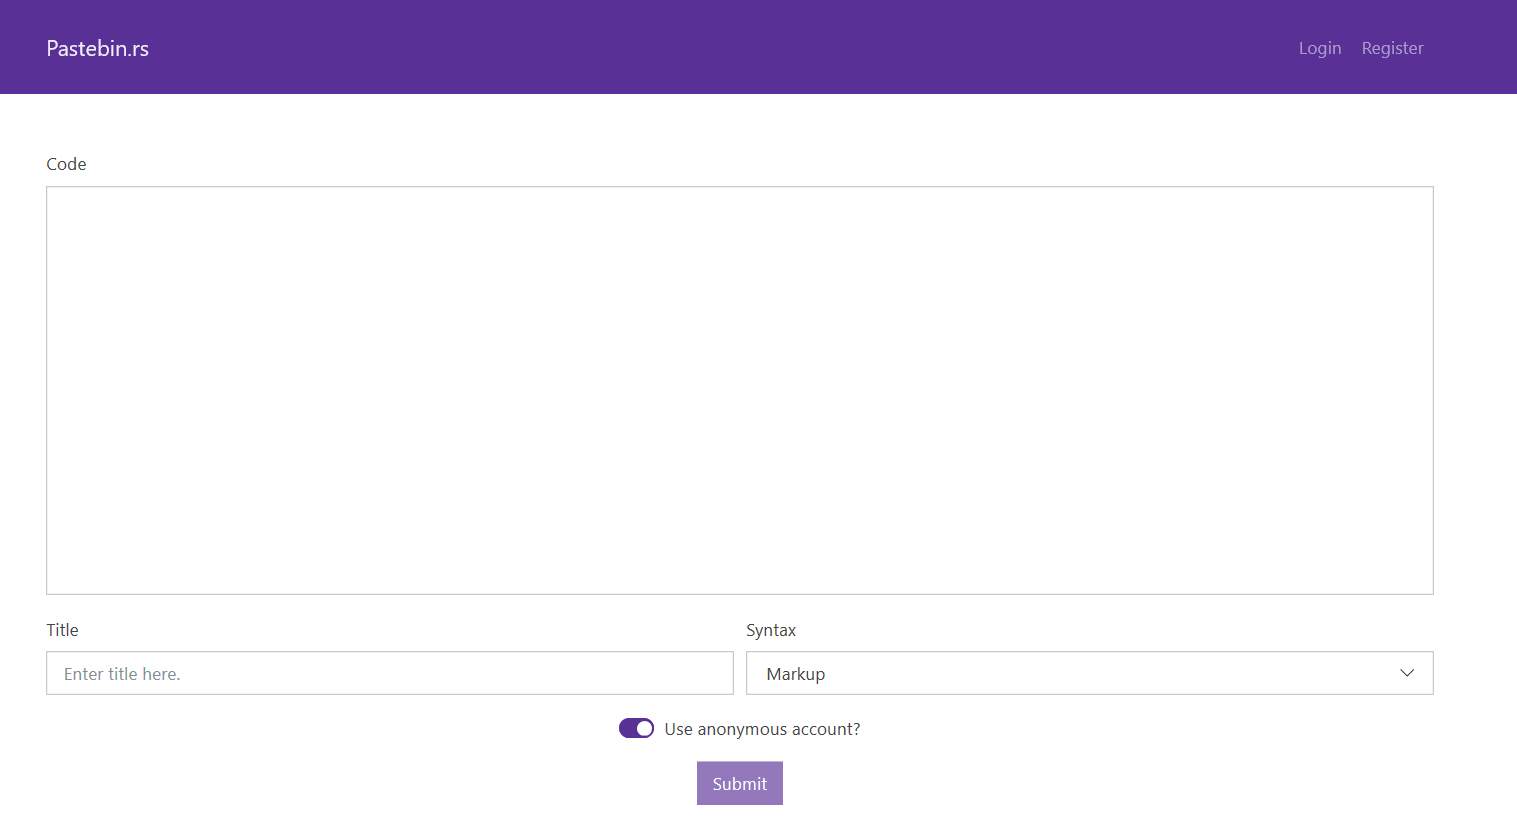
\includegraphics[width=.8\textwidth]{main}
    \caption{主界面}
    \label{fig:main}
\end{figure}

点击左上角登录即可进入登录界面。

\begin{figure}[!htbp]
    \centering
    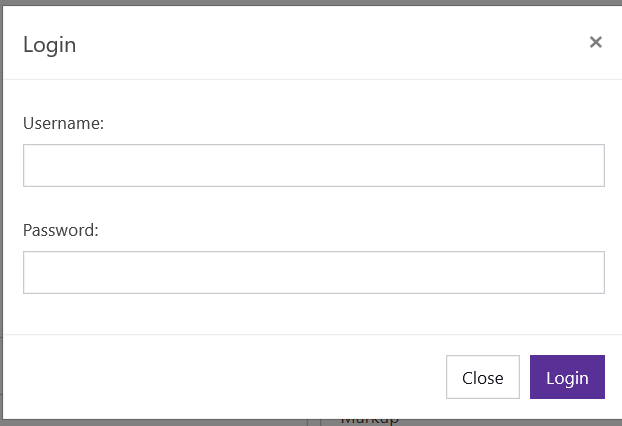
\includegraphics[width=.8\textwidth]{login}
    \caption{登录界面}
    \label{fig:login}
\end{figure}

点击下方的提交按钮即可提交代码,提交后会直接跳转到对应代码的展示界面。点击右上角的用户名,可以进入用户对应的代码片段的展示列表。

\begin{figure}[!htbp]
    \centering
    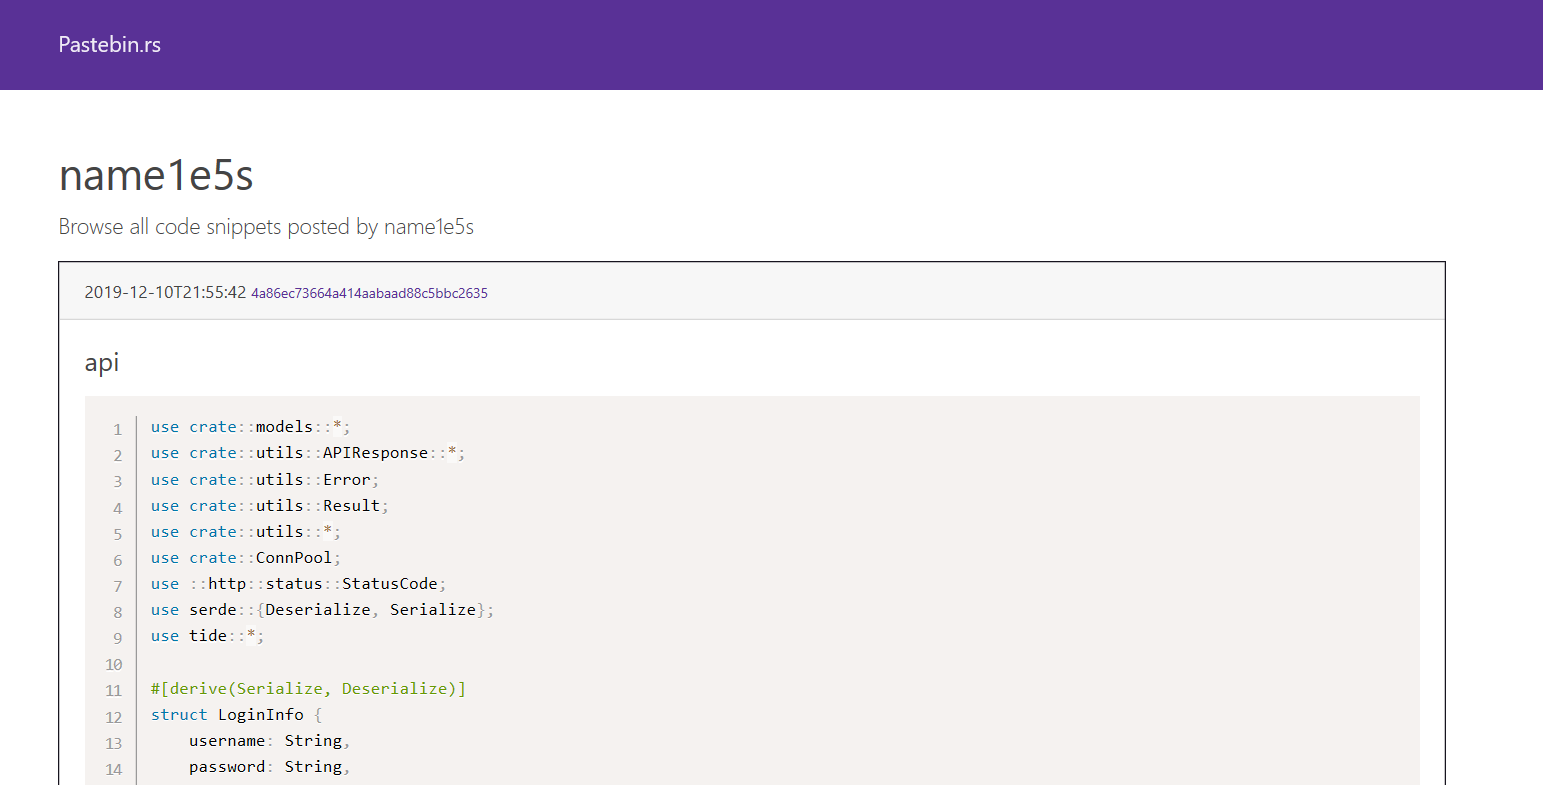
\includegraphics[width=.8\textwidth]{user}
    \caption{用户界面}
    \label{fig:user}
\end{figure}

在列表内点击任一 UUID,即可进入该代码片段对应的展示界面。

\begin{figure}[!htbp]
    \centering
    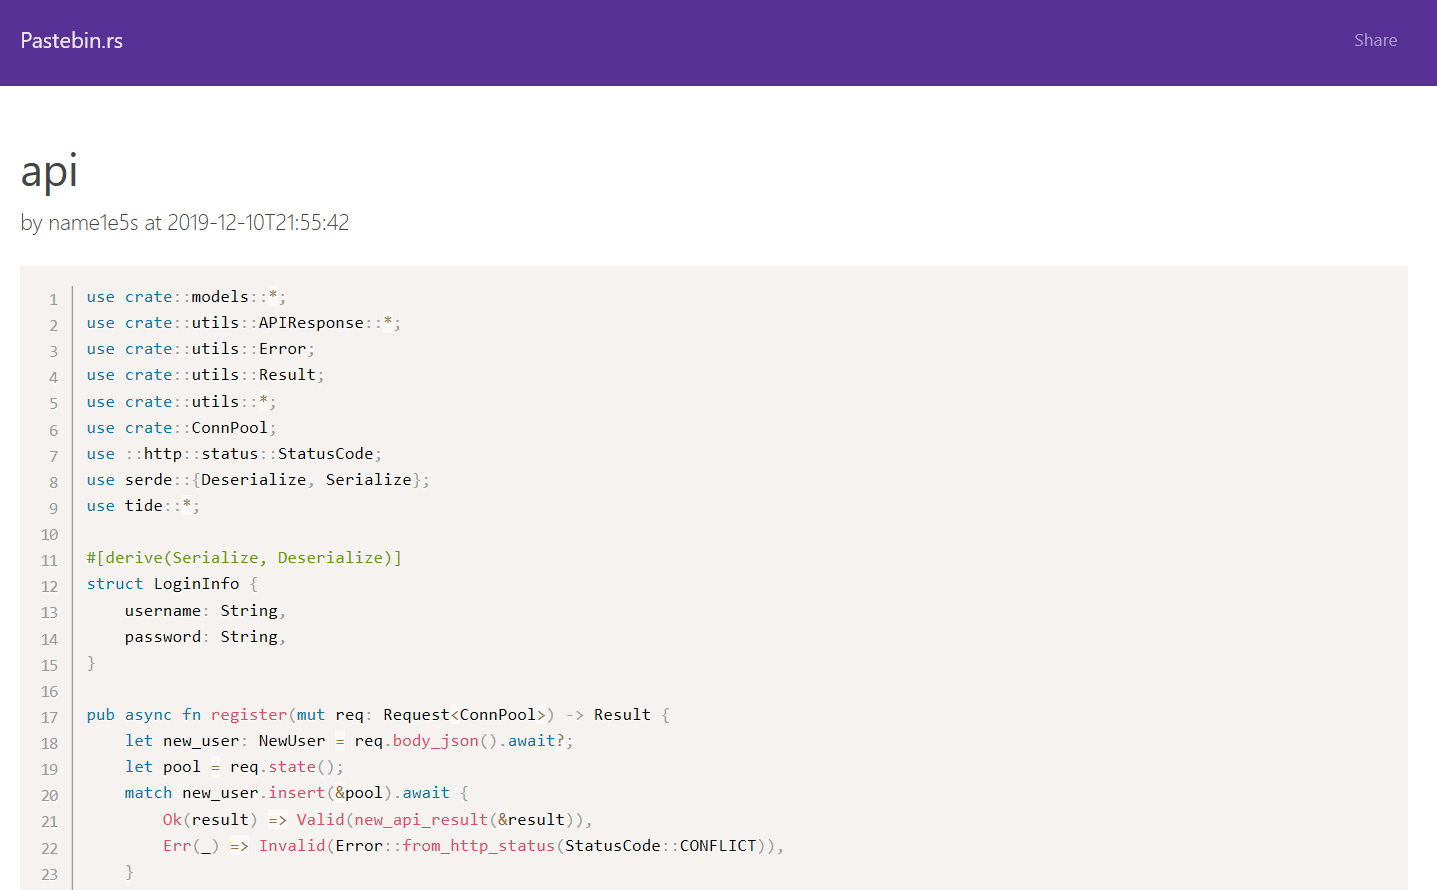
\includegraphics[width=.8\textwidth]{paste}
    \caption{代码片段界面}
    \label{fig:paste}
\end{figure}

点击右上角的 Share,弹出分享窗口,可以在这里复制连接或者获取二维码以供分享。

\begin{figure}[!htbp]
    \centering
    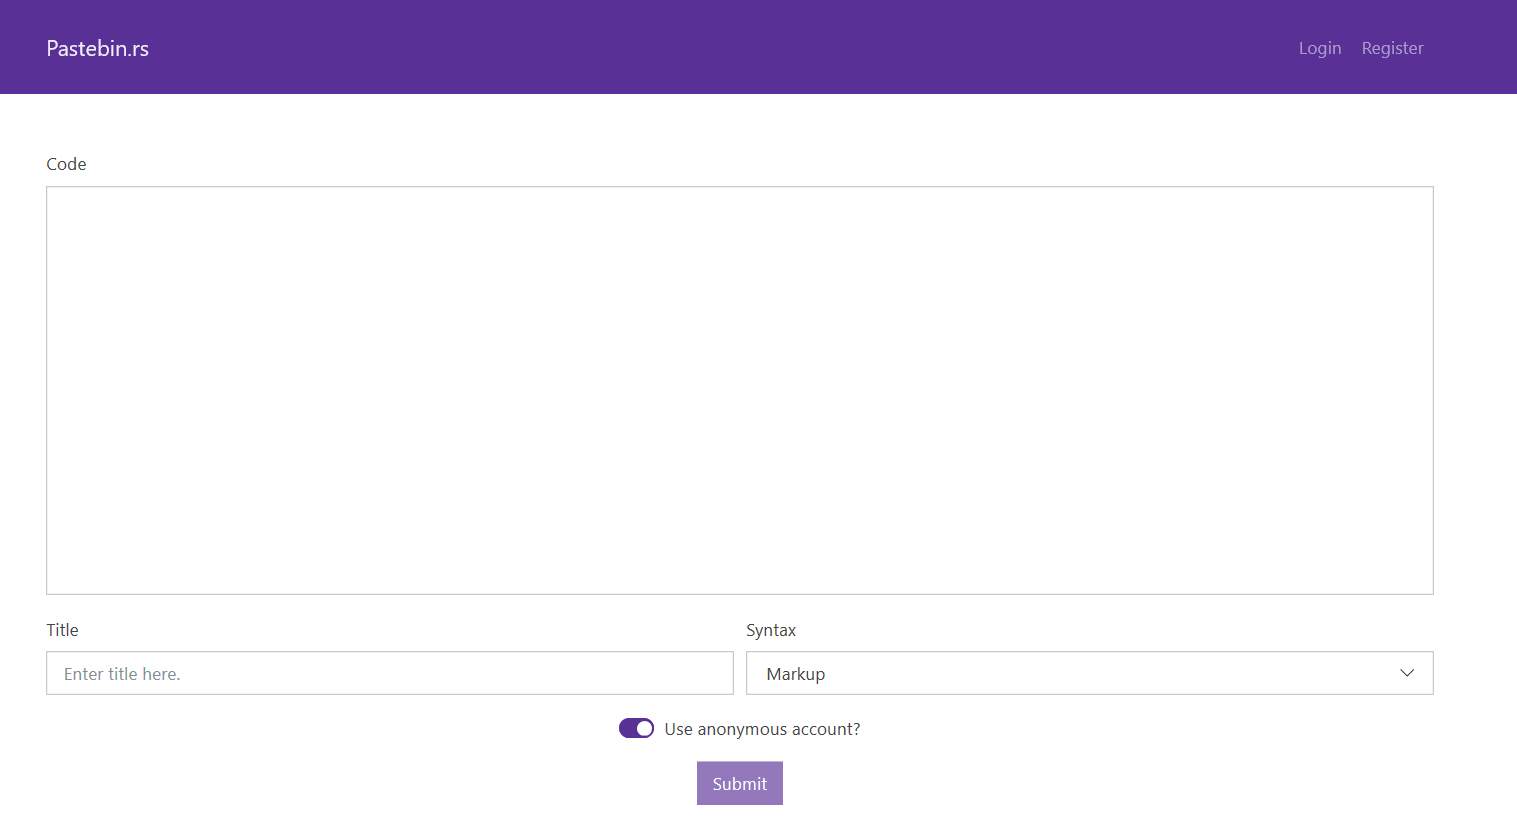
\includegraphics[width=.8\textwidth]{main}
    \caption{分享界面}
    \label{fig:share}
\end{figure}

\section{总结与心得}
本次作业中的需求其实来自个人的亲身经历,有很多时候我都需要将一份代码从装了 Linux 的电脑上转移手机上继续查看或者和别人讨论如何修改,但是没有任何一个应用能提供给我比较合适的体验,作为 Ubuntu Pastebin 也只能是把代码复制出去,然后我去在手机上一个个的输入 BASE 62 后的字符串访问地址,因此我就需要一个能够咸宁市二维码的 Pastebin 方便我进行代码的交换,最好性能还不差。因此我就选择了使用 Rust 去实现一个带有二维码的 Pastebin 来作为程序设计实践课程的作业主题。
这次作业是我第一次使用 Rust 实现有规模的程序,也是第一次完成后端程序的设计。在这次程序设计实践的大作业中我有很多时间都花费在了查找文档以及了解相关知识上。因为对前端的知识一窍不通,所以花了很长时间在如何实现出一个能用的网页上面,很惭愧。不过好在最后实现的程序效果比较完美,也算是比较开心吧。


\end{document}